\chapter{SYSTEM DESIGN}
\label{ch:system_design}

\section{Data Flow Diagram}
\label{sec:dfd}

The functional data architecture and information boundaries of the UniExpert platform are formalized through hierarchical Data Flow Diagrams (DFDs).

\subsection{Data Flow Diagram Level-0}
\label{subsec:dfd_level0}

The Level-0 Context Diagram (Figure~\ref{fig:dfd_level0}) establishes the foundational boundary between the external actors and the centralized UniExpert system. All inbound and outbound data streams are channeled through distinct, dedicated interface vectors.

\begin{figure}[H]
\centering
\begin{tikzpicture}[
    scale=0.88, every node/.style={transform shape},
    font=\sffamily\scriptsize,
    entity/.style={rectangle, draw=black!80, thick, fill=blue!8, align=center, minimum width=2.8cm, minimum height=1.2cm, rounded corners=3pt},
    process/.style={circle, draw=black!80, thick, fill=teal!10, align=center, minimum size=3.6cm, font=\sffamily\bfseries\small},
    arr/.style={-{Stealth[scale=0.9]}, thick, draw=black!70}
]

% Central Process
\node[process] (sys) at (5.5, 0) {0\\Level-0\\UniExpert\\Platform};

% Entities symmetrically placed
\node[entity] (student) at (-1.8, 3.6) {\textbf{Student Project Lead}};
\node[entity] (faculty) at (12.8, 3.6) {\textbf{Faculty Advisor}};
\node[entity] (mentor)  at (-1.8, -3.6) {\textbf{Industry Mentor}};
\node[entity] (coord)   at (12.8, -3.6) {\textbf{Department Coordinator}};
\node[entity] (admin)   at (5.5, 6.2) {\textbf{System Administrator}};
\node[entity] (auditor) at (5.5, -6.2) {\textbf{Institutional Auditor}};

% Student flows (separated parallel paths)
\draw[arr] ([yshift=3pt]student.south east) -- node[above, sloped, font=\tiny] {Problem Statement, Query Sliders} ([yshift=15pt]sys.west);
\draw[arr] ([yshift=-15pt]sys.west) -- node[below, sloped, font=\tiny] {Ranked Advisors, XAI Explanation Cards} ([yshift=-3pt]student.south east);

% Faculty flows (separated parallel paths)
\draw[arr] ([yshift=3pt]faculty.south west) -- node[above, sloped, font=\tiny] {Scholar Metadata, Quotas, FSM Decision} ([yshift=15pt]sys.east);
\draw[arr] ([yshift=-15pt]sys.east) -- node[below, sloped, font=\tiny] {Advisory Proposals, Meeting Invites} ([yshift=-3pt]faculty.south west);

% Mentor flows (separated parallel paths)
\draw[arr] ([yshift=3pt]mentor.north east) -- node[above, sloped, font=\tiny] {Practitioner Credentials, Availability} ([yshift=-15pt]sys.west);
\draw[arr] ([yshift=-35pt]sys.west) -- node[below, sloped, font=\tiny] {Mentorship Invites, Milestone Drafts} ([yshift=-12pt]mentor.north east);

% Coordinator flows (separated parallel paths)
\draw[arr] ([yshift=3pt]coord.north west) -- node[above, sloped, font=\tiny] {Taxonomy Rules, Quota Policies} ([yshift=-15pt]sys.east);
\draw[arr] ([yshift=-35pt]sys.east) -- node[below, sloped, font=\tiny] {Allocation Heatmaps, Disputed Teams} ([yshift=-12pt]coord.north west);

% Administrator flows (parallel vertical separation with xshift)
\draw[arr] ([xshift=-14pt]admin.south) -- node[left, font=\tiny, align=right] {Auth Scopes,\\Index Maintenance} ([xshift=-14pt]sys.north);
\draw[arr] ([xshift=14pt]sys.north) -- node[right, font=\tiny, align=left] {Audit Logs,\\Health Telemetry} ([xshift=14pt]admin.south);

% Auditor flows (parallel vertical separation with xshift)
\draw[arr] ([xshift=-14pt]auditor.north) -- node[left, font=\tiny, align=right] {Compliance Query,\\Audit Filter Parameters} ([xshift=-14pt]sys.south);
\draw[arr] ([xshift=14pt]sys.south) -- node[right, font=\tiny, align=left] {Accreditation Reports,\\Cryptographic Audit CSVs} ([xshift=14pt]auditor.north);

\end{tikzpicture}
\caption{Data Flow Diagram Level-0 (Context Diagram)}
\label{fig:dfd_level0}
\end{figure}

\clearpage
\subsection{Data Flow Diagram Level-1}
\label{subsec:dfd_level1}

The Level-1 Data Flow Diagram (Figure~\ref{fig:dfd_level1}) decomposes the centralized system into six functional microservice processes and six persistent data repositories, structured into a clean orthogonal pipelined layout.

\begin{figure}[H]
\centering
\begin{tikzpicture}[
    scale=0.76, every node/.style={transform shape},
    font=\sffamily\tiny,
    proc/.style={rectangle, rounded corners=6pt, draw=black!80, thick, fill=teal!8, align=center, minimum width=2.6cm, minimum height=1.1cm},
    store/.style={cylinder, draw=black!80, thick, fill=orange!10, shape border rotate=90, aspect=0.25, minimum width=2.3cm, minimum height=1.0cm, align=center},
    ent/.style={rectangle, draw=black!80, thick, fill=blue!10, align=center, minimum width=2.4cm, minimum height=1.0cm, rounded corners=2pt},
    arr/.style={-{Stealth[scale=0.85]}, thick, draw=black!70}
]

% External Entities at cardinal edges
\node[ent] (e_admin)   at (5.0, 7.2)  {\textbf{System Administrator}};
\node[ent] (e_student) at (-2.4, 1.8) {\textbf{Student Project Lead}};
\node[ent] (e_faculty) at (12.4, 1.8) {\textbf{Faculty Advisor}};
\node[ent] (e_coord)   at (12.4, -4.5) {\textbf{Department Coordinator}};

% Layer 1: Authentication & User DB (y = 5.0)
\node[proc] (p1) at (2.0, 5.0) {1.0 Identity \&\\Session Auth};
\node[store] (d1) at (6.0, 5.0) {D1: User Auth DB\\(PostgreSQL)};

% Layer 2: NLP & Matchmaking (y = 1.8)
\node[proc] (p2) at (2.0, 1.8) {2.0 NLP Parsing \&\\Skill Extractor};
\node[store] (d2) at (2.0, 3.4) {D2: Taxonomy DB};
\node[proc] (p3) at (6.0, 1.8) {3.0 Vector Embedding\\\& Hybrid Ranker};
\node[store] (d3) at (9.6, 1.8) {D3: Dense Vectors\\(Qdrant HNSW)};

% Layer 3: Advisory FSM & Collaboration (y = -1.5)
\node[proc] (p4) at (2.0, -1.5) {4.0 Advisory FSM \&\\Quota Governance};
\node[store] (d4) at (6.0, -1.5) {D4: Advisory Requests\\\& Workspace DB};
\node[proc] (p5) at (9.6, -1.5) {5.0 Consultation Sched.\\\& Availability};

% Layer 4: Audit & Analytics (y = -4.5)
\node[proc] (p6) at (2.0, -4.5) {6.0 Institutional Audit\\\& Analytics Reporting};
\node[store] (d6) at (6.0, -4.5) {D6: Append-Only\\Audit Ledger};
\node[store] (d5) at (9.6, -4.5) {D5: Consultation\\Calendar Store};

% Clean Orthogonal Flows (Zero Intersections)
% Admin to P1
\draw[arr] (e_admin.west) -| (p1.north);
\draw[arr] (p1) -- node[above] {Validate} (d1);

% Student NLP flows
\draw[arr] ([yshift=6pt]e_student.east) -- node[above] {Problem Text} ([yshift=6pt]p2.west);
\draw[arr] ([yshift=-6pt]p2.west) -- node[below] {Ranked Advisors} ([yshift=-6pt]e_student.east);
\draw[arr] (d2) -- (p2);
\draw[arr] (p2) -- node[above] {Parsed Skills} (p3);
\draw[arr] (p3) -- node[above] {ANN Query} (d3);

% Student Proposal & Faculty FSM flows
\draw[arr] (e_student.south) |- (p4.west);
\draw[arr] (p4) -- node[above] {FSM State} (d4);
\draw[arr] (e_faculty.south) |- (p5.east);
\draw[arr] (e_faculty.west) -| (d4.north);

% Consultation & Calendar flows
\draw[arr] (d4) -- (p5);
\draw[arr] (p5) -- node[right] {Persist Slots} (d5);

% Audit & Compliance flows
\draw[arr] (p4) -- node[left] {Events} (p6);
\draw[arr] (p6) -- node[above] {Chained Logs} (d6);
\draw[arr] (p6) -- ++(0, -1.0) -| node[above, near start] {Accreditation Reports} (e_coord.south);

\end{tikzpicture}
\caption{Data Flow Diagram Level-1 (Functional Decomposition)}
\label{fig:dfd_level1}
\end{figure}

\clearpage
\section{Sequence Diagram}
\label{sec:sequence_diagrams}

The dynamic message exchanges, component activations, and lifecycle lifelines across system boundaries are detailed in the six sequence diagrams below.

\subsection{Sequence Diagram-01: Problem Statement Ingestion \& AI Expert Recommendation}
\label{subsec:seq01}

This interaction captures the complete flow from raw natural language input to dense vector similarity matching and composite explainable ranking.

\begin{figure}[H]
\centering
\begin{tikzpicture}[
    scale=0.84, every node/.style={transform shape},
    font=\sffamily\tiny,
    actor/.style={rectangle, draw=black, thick, fill=blue!10, align=center, minimum width=1.8cm, minimum height=0.7cm},
    obj/.style={rectangle, draw=black, thick, fill=gray!10, align=center, minimum width=1.8cm, minimum height=0.7cm},
    lifeline/.style={dashed, thick},
    call/.style={-{Stealth[scale=0.8]}, thick},
    ret/.style={dashed, -{Stealth[scale=0.8]}, thick},
    act/.style={rectangle, fill=white, draw=black, thick, minimum width=0.25cm}
]

% Lifeline Headers
\node[actor] (st) at (0, 0) {Student Lead};
\node[obj] (ui) at (2.4, 0) {:ClientApp};
\node[obj] (gw) at (4.8, 0) {:APIGateway};
\node[obj] (nlp) at (7.2, 0) {:NLPService};
\node[obj] (qd) at (9.6, 0) {:QdrantStore};
\node[obj] (db) at (12.0, 0) {:PostgreSQL};

% Lifelines
\draw[lifeline] (st) -- (0, -8.5);
\draw[lifeline] (ui) -- (2.4, -8.5);
\draw[lifeline] (gw) -- (4.8, -8.5);
\draw[lifeline] (nlp) -- (7.2, -8.5);
\draw[lifeline] (qd) -- (9.6, -8.5);
\draw[lifeline] (db) -- (12.0, -8.5);

% Messages
\draw[call] (0, -1.0) -- node[above] {1. Submit Problem Text} (2.4, -1.0);
\draw[call] (2.4, -1.5) -- node[above] {2. POST /api/v1/projects/parse} (4.8, -1.5);
\draw[call] (4.8, -2.0) -- node[above] {3. Zero-shot \& NER parse} (7.2, -2.0);
\node[act, minimum height=1.2cm] at (7.2, -2.6) {};
\draw[ret] (7.2, -3.2) -- node[above] {4. Extracted Domains \& Skills} (4.8, -3.2);
\draw[ret] (4.8, -3.6) -- node[above] {5. Render Entity Review Card} (2.4, -3.6);
\draw[call] (0, -4.2) -- node[above] {6. Confirm Skills \& Sliders} (2.4, -4.2);
\draw[call] (2.4, -4.6) -- node[above] {7. POST /api/v1/matchmaking/query} (4.8, -4.6);
\draw[call] (4.8, -5.0) -- node[above] {8. Dense Vector Cosine Search} (9.6, -5.0);
\node[act, minimum height=0.8cm] at (9.6, -5.4) {};
\draw[ret] (9.6, -5.8) -- node[above] {9. Top-50 Candidate IDs \& Cosine} (4.8, -5.8);
\draw[call] (4.8, -6.3) -- node[above] {10. Fetch Profiles, Citations \& Quotas} (12.0, -6.3);
\draw[ret] (12.0, -6.8) -- node[above] {11. Relational Profile Attributes} (4.8, -6.8);
\draw[ret] (4.8, -7.4) -- node[above] {12. Composite Rank + XAI Payloads} (2.4, -7.4);
\draw[ret] (2.4, -7.9) -- node[above] {13. Display Ranked Advisor List} (0, -7.9);

\end{tikzpicture}
\caption{Sequence Diagram for Problem Ingestion \& AI Recommendation}
\label{fig:seq_problem_match}
\end{figure}

\clearpage
\subsection{Sequence Diagram-02: Advisory Collaboration Request \& FSM Lifecycle Negotiation}
\label{subsec:seq02}

This sequence models the asynchronous multi-party negotiation protocol between the Student Project Lead and the Faculty Advisor through the state-machine manager.

\begin{figure}[H]
\centering
\begin{tikzpicture}[
    scale=0.84, every node/.style={transform shape},
    font=\sffamily\tiny,
    actor/.style={rectangle, draw=black, thick, fill=blue!10, align=center, minimum width=1.8cm, minimum height=0.7cm},
    obj/.style={rectangle, draw=black, thick, fill=gray!10, align=center, minimum width=1.8cm, minimum height=0.7cm},
    lifeline/.style={dashed, thick},
    call/.style={-{Stealth[scale=0.8]}, thick},
    ret/.style={dashed, -{Stealth[scale=0.8]}, thick},
    act/.style={rectangle, fill=white, draw=black, thick, minimum width=0.25cm}
]

\node[actor] (st) at (0, 0) {Student Lead};
\node[obj] (gw) at (3.0, 0) {:APIGateway};
\node[obj] (fsm) at (6.0, 0) {:FSMService};
\node[actor] (fa) at (9.0, 0) {Faculty Advisor};
\node[obj] (db) at (12.0, 0) {:PostgreSQL};

\draw[lifeline] (st) -- (0, -8.0);
\draw[lifeline] (gw) -- (3.0, -8.0);
\draw[lifeline] (fsm) -- (6.0, -8.0);
\draw[lifeline] (fa) -- (9.0, -8.0);
\draw[lifeline] (db) -- (12.0, -8.0);

\draw[call] (0, -1.0) -- node[above] {1. Submit Advisory Proposal} (3.0, -1.0);
\draw[call] (3.0, -1.5) -- node[above] {2. Transition: DRAFT $\rightarrow$ SUBMITTED} (6.0, -1.5);
\draw[call] (6.0, -2.0) -- node[above] {3. Verify Quota Capacity ($\ge 1$)} (12.0, -2.0);
\draw[ret] (12.0, -2.5) -- node[above] {4. Quota Validated; Request Saved} (6.0, -2.5);
\draw[call] (6.0, -3.0) -- node[above] {5. Push Proposal Alert Notification} (9.0, -3.0);
\draw[call] (9.0, -3.7) -- node[above] {6. Open Proposal (Status $\rightarrow$ UNDER\_REVIEW)} (6.0, -3.7);
\draw[call] (9.0, -4.5) -- node[above] {7. Request Scope Revisions (NEGOTIATION)} (6.0, -4.5);
\draw[call] (6.0, -5.0) -- node[above] {8. Alert Student of Requested Revisions} (0, -5.0);
\draw[call] (0, -5.7) -- node[above] {9. Re-submit Revised Milestone Plan} (6.0, -5.7);
\draw[call] (9.0, -6.4) -- node[above] {10. Accept Proposal (Status $\rightarrow$ ACCEPTED)} (6.0, -6.4);
\draw[call] (6.0, -7.0) -- node[above] {11. Decrement Faculty Quota \& Init Workspace} (12.0, -7.0);
\draw[ret] (6.0, -7.6) -- node[above] {12. Notify Confirmation to All Parties} (0, -7.6);

\end{tikzpicture}
\caption{Sequence Diagram for Advisory Request FSM Lifecycle}
\label{fig:seq_fsm}
\end{figure}

\clearpage
\subsection{Sequence Diagram-03: Expert Profile Ingestion \& Dense Vector Indexing}
\label{subsec:seq03}

This sequence details the asynchronous ingestion of academic publications via external Scholar and ORCID APIs, followed by embedding generation and vector upsert.

\begin{figure}[H]
\centering
\begin{tikzpicture}[
    scale=0.84, every node/.style={transform shape},
    font=\sffamily\tiny,
    actor/.style={rectangle, draw=black, thick, fill=teal!10, align=center, minimum width=1.8cm, minimum height=0.7cm},
    obj/.style={rectangle, draw=black, thick, fill=gray!10, align=center, minimum width=1.8cm, minimum height=0.7cm},
    lifeline/.style={dashed, thick},
    call/.style={-{Stealth[scale=0.8]}, thick},
    ret/.style={dashed, -{Stealth[scale=0.8]}, thick},
    act/.style={rectangle, fill=white, draw=black, thick, minimum width=0.25cm}
]

\node[actor] (fa) at (0, 0) {Faculty Advisor};
\node[obj] (ui) at (2.4, 0) {:ClientApp};
\node[obj] (gw) at (4.8, 0) {:APIGateway};
\node[obj] (ext) at (7.2, 0) {:Scholar/ORCID API};
\node[obj] (embed) at (9.6, 0) {:EmbeddingWorker};
\node[obj] (qd) at (12.0, 0) {:QdrantStore};

\draw[lifeline] (fa) -- (0, -7.5);
\draw[lifeline] (ui) -- (2.4, -7.5);
\draw[lifeline] (gw) -- (4.8, -7.5);
\draw[lifeline] (ext) -- (7.2, -7.5);
\draw[lifeline] (embed) -- (9.6, -7.5);
\draw[lifeline] (qd) -- (12.0, -7.5);

\draw[call] (0, -1.0) -- node[above] {1. Enter ORCID / Scholar Profile ID} (2.4, -1.0);
\draw[call] (2.4, -1.5) -- node[above] {2. POST /api/v1/profile/sync} (4.8, -1.5);
\draw[call] (4.8, -2.0) -- node[above] {3. Query Publications \& Abstracts} (7.2, -2.0);
\node[act, minimum height=0.9cm] at (7.2, -2.4) {};
\draw[ret] (7.2, -2.9) -- node[above] {4. Ingest Paper Metadata \& Citations} (4.8, -2.9);
\draw[call] (4.8, -3.5) -- node[above] {5. Enqueue Embedding Task} (9.6, -3.5);
\node[act, minimum height=1.2cm] at (9.6, -4.0) {};
% Proper looping self-call
\draw[call] (9.6, -4.5) -- ++(1.2, 0) -- ++(0, -0.6) -- node[above, right=2pt, font=\tiny] {6. Generate 384-d Dense Vector} ++(-1.2, 0);
\draw[call] (9.6, -5.5) -- node[above] {7. Upsert Vector with Payload} (12.0, -5.5);
\draw[ret] (12.0, -6.1) -- node[above] {8. Index Confirmation (HNSW)} (9.6, -6.1);
\draw[ret] (9.6, -6.6) -- node[above] {9. Task Completed} (4.8, -6.6);
\draw[ret] (4.8, -7.1) -- node[above] {10. Display Profile Verified \& Synced} (0, -7.1);

\end{tikzpicture}
\caption{Sequence Diagram for Expert Profile Ingestion \& Vector Indexing}
\label{fig:seq_profile_sync}
\end{figure}

\clearpage
\subsection{Sequence Diagram-04: Multidisciplinary Team Skill Gap Analysis \& Co-Advisor Discovery}
\label{subsec:seq04}

This sequence shows the calculation of skill deficits ($\Delta\mathcal{K}$) and the set-cover optimization that suggests co-advisors across different departments.

\begin{figure}[H]
\centering
\begin{tikzpicture}[
    scale=0.84, every node/.style={transform shape},
    font=\sffamily\tiny,
    actor/.style={rectangle, draw=black, thick, fill=blue!10, align=center, minimum width=1.8cm, minimum height=0.7cm},
    obj/.style={rectangle, draw=black, thick, fill=gray!10, align=center, minimum width=1.8cm, minimum height=0.7cm},
    lifeline/.style={dashed, thick},
    call/.style={-{Stealth[scale=0.8]}, thick},
    ret/.style={dashed, -{Stealth[scale=0.8]}, thick},
    act/.style={rectangle, fill=white, draw=black, thick, minimum width=0.25cm}
]

\node[actor] (st) at (0, 0) {Student Lead};
\node[obj] (gw) at (3.0, 0) {:APIGateway};
\node[obj] (gap) at (6.0, 0) {:SkillGapEngine};
\node[obj] (opt) at (9.0, 0) {:SetCoverOptimizer};
\node[obj] (db) at (12.0, 0) {:PostgreSQL};

\draw[lifeline] (st) -- (0, -7.5);
\draw[lifeline] (gw) -- (3.0, -7.5);
\draw[lifeline] (gap) -- (6.0, -7.5);
\draw[lifeline] (opt) -- (9.0, -7.5);
\draw[lifeline] (db) -- (12.0, -7.5);

\draw[call] (0, -1.0) -- node[above] {1. Click ``Analyze Skill Gaps''} (3.0, -1.0);
\draw[call] (3.0, -1.5) -- node[above] {2. Fetch Required Skills \& Team Roster} (12.0, -1.5);
\draw[ret] (12.0, -2.1) -- node[above] {3. Return $\mathcal{K}_{\text{req}}$ and $\mathcal{K}_{\text{team}}$} (3.0, -2.1);
\draw[call] (3.0, -2.6) -- node[above] {4. Compute Deficit: $\Delta \mathcal{K} = \mathcal{K}_{\text{req}} \setminus \mathcal{K}_{\text{team}}$} (6.0, -2.6);
\node[act, minimum height=0.8cm] at (6.0, -3.0) {};
\draw[call] (6.0, -3.5) -- node[above] {5. Invoke Set-Cover on External Departments} (9.0, -3.5);
\node[act, minimum height=1.0cm] at (9.0, -4.0) {};
\draw[call] (9.0, -4.5) -- node[above] {6. Query Faculty Covering Deficits} (12.0, -4.5);
\draw[ret] (12.0, -5.1) -- node[above] {7. Candidate Faculty Profiles} (9.0, -5.1);
\draw[ret] (9.0, -5.7) -- node[above] {8. Minimal Co-Advisor Recommendation Set} (3.0, -5.7);
\draw[ret] (3.0, -6.4) -- node[above] {9. Render Skill Deficit Card \& Co-Advisors} (0, -6.4);
\draw[call] (0, -7.0) -- node[above] {10. Propose Multidisciplinary Co-Advisory} (3.0, -7.0);

\end{tikzpicture}
\caption{Sequence Diagram for Multidisciplinary Skill Gap Optimization}
\label{fig:seq_skill_gap}
\end{figure}

\clearpage
\subsection{Sequence Diagram-05: Mentorship Consultation Scheduling \& Availability Check}
\label{subsec:seq05}

This sequence demonstrates the race-free booking of faculty and industry mentor office hours through atomic database row-locking.

\begin{figure}[H]
\centering
\begin{tikzpicture}[
    scale=0.84, every node/.style={transform shape},
    font=\sffamily\tiny,
    actor/.style={rectangle, draw=black, thick, fill=blue!10, align=center, minimum width=1.8cm, minimum height=0.7cm},
    obj/.style={rectangle, draw=black, thick, fill=gray!10, align=center, minimum width=1.8cm, minimum height=0.7cm},
    lifeline/.style={dashed, thick},
    call/.style={-{Stealth[scale=0.8]}, thick},
    ret/.style={dashed, -{Stealth[scale=0.8]}, thick},
    act/.style={rectangle, fill=white, draw=black, thick, minimum width=0.25cm}
]

\node[actor] (st) at (0, 0) {Student Lead};
\node[obj] (ui) at (3.0, 0) {:ClientApp};
\node[obj] (sched) at (6.0, 0) {:SchedulerService};
\node[actor] (fa) at (9.0, 0) {Faculty Advisor};
\node[obj] (db) at (12.0, 0) {:PostgreSQL};

\draw[lifeline] (st) -- (0, -7.5);
\draw[lifeline] (ui) -- (3.0, -7.5);
\draw[lifeline] (sched) -- (6.0, -7.5);
\draw[lifeline] (fa) -- (9.0, -7.5);
\draw[lifeline] (db) -- (12.0, -7.5);

\draw[call] (9.0, -0.8) -- node[above] {1. Publish Office Hours \& Capacity} (6.0, -0.8);
\draw[call] (6.0, -1.3) -- node[above] {2. Persist Available Time Slots} (12.0, -1.3);
\draw[call] (0, -2.0) -- node[above] {3. Request Advisor Consultation Calendar} (3.0, -2.0);
\draw[call] (3.0, -2.5) -- node[above] {4. GET /api/v1/advisors/\{id\}/slots} (6.0, -2.5);
\draw[ret] (6.0, -3.0) -- node[above] {5. Return Open 30-min Slots} (3.0, -3.0);
\draw[call] (0, -3.8) -- node[above] {6. Select Slot \& Enter Agenda} (3.0, -3.8);
\draw[call] (3.0, -4.3) -- node[above] {7. POST /api/v1/consultations/book} (6.0, -4.3);
\draw[call] (6.0, -4.9) -- node[above] {8. Atomic Row Lock: Verify \& Claim Slot} (12.0, -4.9);
\node[act, minimum height=0.8cm] at (12.0, -5.3) {};
\draw[ret] (12.0, -5.7) -- node[above] {9. Slot Confirmed as BOOKED} (6.0, -5.7);
\draw[call] (6.0, -6.3) -- node[above] {10. Dispatch iCal Invite \& Email Alert} (9.0, -6.3);
\draw[ret] (6.0, -6.8) -- node[above] {11. Booking Confirmation \& Meeting Link} (0, -6.8);

\end{tikzpicture}
\caption{Sequence Diagram for Consultation Scheduling}
\label{fig:seq_consultation}
\end{figure}

\clearpage
\subsection{Sequence Diagram-06: Institutional Compliance Audit Search \& Export}
\label{subsec:seq06}

This sequence shows the tamper-evident query verification mechanism used by coordinators and auditors to inspect cryptographically chained audit trails.

\begin{figure}[H]
\centering
\begin{tikzpicture}[
    scale=0.84, every node/.style={transform shape},
    font=\sffamily\tiny,
    actor/.style={rectangle, draw=black, thick, fill=purple!10, align=center, minimum width=1.8cm, minimum height=0.7cm},
    obj/.style={rectangle, draw=black, thick, fill=gray!10, align=center, minimum width=1.8cm, minimum height=0.7cm},
    lifeline/.style={dashed, thick},
    call/.style={-{Stealth[scale=0.8]}, thick},
    ret/.style={dashed, -{Stealth[scale=0.8]}, thick},
    act/.style={rectangle, fill=white, draw=black, thick, minimum width=0.25cm}
]

\node[actor] (aud) at (0, 0) {Auditor / Coord};
\node[obj] (ui) at (3.0, 0) {:ClientApp};
\node[obj] (gw) at (6.0, 0) {:APIGateway};
\node[obj] (audit) at (9.0, 0) {:AuditService};
\node[obj] (db) at (12.0, 0) {:Append-Only DB};

\draw[lifeline] (aud) -- (0, -7.5);
\draw[lifeline] (ui) -- (3.0, -7.5);
\draw[lifeline] (gw) -- (6.0, -7.5);
\draw[lifeline] (audit) -- (9.0, -7.5);
\draw[lifeline] (db) -- (12.0, -7.5);

\draw[call] (0, -1.0) -- node[above] {1. Input Filter (Dept, Term, EventType)} (3.0, -1.0);
\draw[call] (3.0, -1.5) -- node[above] {2. GET /api/v1/governance/audit-logs} (6.0, -1.5);
\draw[call] (6.0, -2.0) -- node[above] {3. Forward Query with Auditor Scopes} (9.0, -2.0);
\draw[call] (9.0, -2.5) -- node[above] {4. Execute Filter Query on Audit Tables} (12.0, -2.5);
\draw[ret] (12.0, -3.1) -- node[above] {5. Return Log Entries with Hash Signatures} (9.0, -3.1);
% Proper looping self-call
\draw[call] (9.0, -3.6) -- ++(1.2, 0) -- ++(0, -0.6) -- node[above, right=2pt, font=\tiny] {6. Verify SHA-256 Hash Chain} ++(-1.2, 0);
\draw[ret] (9.0, -4.5) -- node[above] {7. Validated Audit Stream Payload} (6.0, -4.5);
\draw[ret] (6.0, -5.0) -- node[above] {8. Render Interactive Log Table} (3.0, -5.0);
\draw[call] (0, -5.6) -- node[above] {9. Click ``Export Signed Compliance CSV''} (3.0, -5.6);
\draw[call] (3.0, -6.1) -- node[above] {10. Generate Signed Export File} (9.0, -6.1);
\draw[ret] (9.0, -6.7) -- node[above] {11. Download Certified CSV Report} (0, -6.7);

\end{tikzpicture}
\caption{Sequence Diagram for Institutional Compliance Audit Search}
\label{fig:seq_audit}
\end{figure}

\clearpage
\section{State Diagram}
\label{sec:state_diagrams}

The discrete behavioral states, transition triggers, guard conditions, and exit actions governing entities in the UniExpert platform are captured in the six state diagrams below.

\subsection{State Diagram-01: Advisory Request FSM Lifecycle}
\label{subsec:state01}

\begin{figure}[H]
\centering
\begin{tikzpicture}[
    scale=0.88, every node/.style={transform shape},
    font=\sffamily\scriptsize,
    startstop/.style={circle, fill=black, inner sep=4pt},
    state/.style={rectangle, rounded corners=6pt, draw=black!80, thick, fill=teal!8, align=center, minimum width=2.4cm, minimum height=0.9cm},
    final/.style={circle, draw=black, thick, fill=black, inner sep=3pt, double=white, double distance=2pt},
    arrow/.style={-{Stealth[scale=0.9]}, thick, draw=black!70}
]

\node[startstop] (s0) at (0, 0) {};
\node[state] (draft) at (2.2, 0) {Draft};
\node[state] (sub) at (5.2, 0) {Submitted};
\node[state] (rev) at (8.5, 0) {Under Review};
\node[state] (neg) at (8.5, -2.0) {Negotiation};
\node[state] (acc) at (12.0, 0) {Accepted};
\node[state] (dec) at (8.5, 2.0) {Declined};
\node[state] (exp) at (5.2, 2.0) {Expired};

% Distinct terminal nodes for completed vs terminated lifecycle (Zero Line Overlaps)
\node[final] (end_done) at (12.0, -2.0) {};
\node[final] (end_term) at (12.0, 2.0) {};

% Primary Acceptance Pipeline
\draw[arrow] (s0) -- (draft);
\draw[arrow] (draft) -- node[above, font=\tiny] {submitProposal} (sub);
\draw[arrow] (sub) -- node[above, font=\tiny] {openRequest} (rev);
\draw[arrow] (rev) -- node[above, font=\tiny] {accept [quota>0]} (acc);
\draw[arrow] (acc) -- node[right, font=\tiny] {completeCapstone} (end_done);

% Revision Negotiation Loop
\draw[arrow] (rev) -- node[right, font=\tiny] {requestRevisions} (neg);
\draw[arrow] (neg) -| node[left, font=\tiny, near start] {reSubmit} (sub);

% Expiration & Decline Branch (Clean top horizontal routing)
\draw[arrow] (sub) -- node[left, font=\tiny] {timer > 7d} (exp);
\draw[arrow] (exp) -- (dec);
\draw[arrow] (rev) -- node[left, font=\tiny] {decline} (dec);
\draw[arrow] (dec) -- (end_term);

\end{tikzpicture}
\caption{State Diagram for Advisory Request FSM Lifecycle}
\label{fig:state_fsm}
\end{figure}

\bigskip
\subsection{State Diagram-02: User Account Status}
\label{subsec:state02}

\begin{figure}[H]
\centering
\begin{tikzpicture}[
    scale=0.88, every node/.style={transform shape},
    font=\sffamily\scriptsize,
    startstop/.style={circle, fill=black, inner sep=4pt},
    state/.style={rectangle, rounded corners=6pt, draw=black!80, thick, fill=blue!8, align=center, minimum width=2.6cm, minimum height=0.9cm},
    final/.style={circle, draw=black, thick, fill=black, inner sep=3pt, double=white, double distance=2pt},
    arrow/.style={-{Stealth[scale=0.9]}, thick, draw=black!70}
]

\node[startstop] (s0) at (0, 0) {};
\node[state] (pending) at (2.5, 0) {Pending Verification};
\node[state] (active)  at (6.5, 0) {Active Verified};
\node[state] (locked)  at (6.5, 2.2) {Locked (15 min)};
\node[state] (deact)   at (6.5, -2.2) {Suspended / Deactivated};
\node[final] (end)     at (10.5, 0) {};

\draw[arrow] (s0) -- (pending);
\draw[arrow] (pending) -- node[above, font=\tiny] {verifyEmailToken} (active);

% Parallel vertical paths between active and locked (Zero Collisions)
\draw[arrow] ([xshift=-12pt]active.north) -- node[left, font=\tiny] {failedLogins == 5} ([xshift=-12pt]locked.south);
\draw[arrow] ([xshift=12pt]locked.south) -- node[right, font=\tiny] {timerExpires / reset} ([xshift=12pt]active.north);

\draw[arrow] (active) -- node[right, font=\tiny] {adminSuspension / leftUniv} (deact);
\draw[arrow] (active) -- node[above, font=\tiny] {accountPurged} (end);
\draw[arrow] (deact) -| (end);

\end{tikzpicture}
\caption{State Diagram for User Account Status}
\label{fig:state_user}
\end{figure}

\clearpage
\subsection{State Diagram-03: Faculty Advisory Quota \& Availability State}
\label{subsec:state03}

\begin{figure}[H]
\centering
\begin{tikzpicture}[
    scale=0.88, every node/.style={transform shape},
    font=\sffamily\scriptsize,
    startstop/.style={circle, fill=black, inner sep=4pt},
    state/.style={rectangle, rounded corners=6pt, draw=black!80, thick, fill=green!8, align=center, minimum width=2.8cm, minimum height=0.9cm},
    final/.style={circle, draw=black, thick, fill=black, inner sep=3pt, double=white, double distance=2pt},
    arrow/.style={-{Stealth[scale=0.9]}, thick, draw=black!70}
]

\node[startstop] (s0) at (0, 0) {};
\node[state] (avail) at (3.0, 0) {Available ($S_{\text{avail}}=1.0$)};
\node[state] (near)  at (7.5, 0) {Nearing Quota ($S_{\text{avail}}=0.7$)};
\node[state] (full)  at (12.0, 0) {Quota Reached ($S_{\text{avail}}=0$)};
\node[state] (black) at (7.5, -2.0) {Blackout / Sabbatical};
\node[final] (end)   at (12.0, -2.0) {};

\draw[arrow] (s0) -- (avail);
\draw[arrow] ([yshift=4pt]avail.east) -- node[above, font=\tiny] {active == max - 1} ([yshift=4pt]near.west);
\draw[arrow] ([yshift=-4pt]near.west) -- node[below, font=\tiny] {groupCompleted} ([yshift=-4pt]avail.east);
\draw[arrow] ([yshift=4pt]near.east) -- node[above, font=\tiny] {active == max} ([yshift=4pt]full.west);
\draw[arrow] ([yshift=-4pt]full.west) -- node[below, font=\tiny] {groupCompleted} ([yshift=-4pt]near.east);
\draw[arrow] (avail) |- node[left, font=\tiny, near start] {setBlackoutDates} (black);
\draw[arrow] (black) -| node[right, font=\tiny, near end] {blackoutEnded} (avail);
\draw[arrow] (full) -- (end);

\end{tikzpicture}
\caption{State Diagram for Faculty Advisory Quota Availability}
\label{fig:state_quota}
\end{figure}

\bigskip
\subsection{State Diagram-04: Capstone Project Stage Lifecycle}
\label{subsec:state04}

\begin{figure}[H]
\centering
\begin{tikzpicture}[
    scale=0.88, every node/.style={transform shape},
    font=\sffamily\scriptsize,
    startstop/.style={circle, fill=black, inner sep=4pt},
    state/.style={rectangle, rounded corners=6pt, draw=black!80, thick, fill=purple!8, align=center, minimum width=2.6cm, minimum height=0.9cm},
    final/.style={circle, draw=black, thick, fill=black, inner sep=3pt, double=white, double distance=2pt},
    arrow/.style={-{Stealth[scale=0.9]}, thick, draw=black!70}
]

\node[startstop] (s0) at (0, 0) {};
\node[state] (form)    at (2.5, 0) {Problem Formulation};
\node[state] (match)   at (6.0, 0) {Advisor Matching};
\node[state] (active)  at (9.5, 0) {Active Supervision};
\node[state] (defense) at (9.5, -2.0) {Defense Ready};
\node[state] (arch)    at (5.0, -2.0) {Completed \& Archived};
\node[final] (end)     at (1.5, -2.0) {};

\draw[arrow] (s0) -- (form);
\draw[arrow] (form) -- node[above, font=\tiny] {nlpParsed} (match);
\draw[arrow] (match) -- node[above, font=\tiny] {advisorAccepted} (active);
\draw[arrow] (active) -- node[right, font=\tiny] {milestonesApproved} (defense);
\draw[arrow] (defense) -- node[above, font=\tiny] {passDefense \& evaluate} (arch);
\draw[arrow] (arch) -- node[above, font=\tiny] {retentionPurge} (end);

\end{tikzpicture}
\caption{State Diagram for Capstone Project Stage Lifecycle}
\label{fig:state_project}
\end{figure}

\clearpage
\subsection{State Diagram-05: AI Inference \& Matchmaking Pipeline Status}
\label{subsec:state05}

\begin{figure}[H]
\centering
\begin{tikzpicture}[
    scale=0.88, every node/.style={transform shape},
    font=\sffamily\scriptsize,
    startstop/.style={circle, fill=black, inner sep=4pt},
    state/.style={rectangle, rounded corners=6pt, draw=black!80, thick, fill=orange!8, align=center, minimum width=2.6cm, minimum height=0.9cm},
    final/.style={circle, draw=black, thick, fill=black, inner sep=3pt, double=white, double distance=2pt},
    arrow/.style={-{Stealth[scale=0.9]}, thick, draw=black!70}
]

\node[startstop] (s0) at (0, 0) {};
\node[state] (ingest) at (2.5, 0) {Statement Ingested};
\node[state] (ner)    at (6.0, 0) {Entities Extracted};
\node[state] (vec)    at (9.5, 0) {Vectors Retrieved};
\node[state] (rank)   at (9.5, -2.0) {Scored \& Ranked};
\node[state] (xai)    at (5.0, -2.0) {XAI Generated};
\node[final] (end)    at (1.5, -2.0) {};

\draw[arrow] (s0) -- (ingest);
\draw[arrow] (ingest) -- node[above, font=\tiny] {zeroShotNER} (ner);
\draw[arrow] (ner) -- node[above, font=\tiny] {embedQuery \& ANN} (vec);
\draw[arrow] (vec) -- node[right, font=\tiny] {multiCriteriaRank} (rank);
\draw[arrow] (rank) -- node[above, font=\tiny] {xaiDecompose} (xai);
\draw[arrow] (xai) -- node[above, font=\tiny] {deliverResponse} (end);

\end{tikzpicture}
\caption{State Diagram for AI Matchmaking Inference Pipeline}
\label{fig:state_inference}
\end{figure}

\bigskip
\subsection{State Diagram-06: Credential Attestation \& Endorsement Status}
\label{subsec:state06}

\begin{figure}[H]
\centering
\begin{tikzpicture}[
    scale=0.88, every node/.style={transform shape},
    font=\sffamily\scriptsize,
    startstop/.style={circle, fill=black, inner sep=4pt},
    state/.style={rectangle, rounded corners=6pt, draw=black!80, thick, fill=teal!8, align=center, minimum width=2.8cm, minimum height=0.9cm},
    final/.style={circle, draw=black, thick, fill=black, inner sep=3pt, double=white, double distance=2pt},
    arrow/.style={-{Stealth[scale=0.9]}, thick, draw=black!70}
]

\node[startstop] (s0) at (0, 0) {};
\node[state] (unver) at (2.8, 0) {Tier-0 (Unverified)};
\node[state] (t1)    at (6.8, 0) {Tier-1 (Domain Verified)};
\node[state] (t2)    at (11.0, 0) {Tier-2 (Scholar Synced)};
\node[state] (t3)    at (8.5, -2.0) {Tier-3 (Chair Validated)};
\node[final] (end)   at (12.5, -2.0) {};

\draw[arrow] (s0) -- (unver);
\draw[arrow] (unver) -- node[above, font=\tiny] {verifyEmailToken} (t1);
\draw[arrow] (t1) -- node[above, font=\tiny] {syncORCID / Scholar} (t2);
\draw[arrow] (t2) |- node[left, font=\tiny, near start] {chairReviewApproved} (t3);
\draw[arrow] (t2) -- node[right, font=\tiny] {active} (end);
\draw[arrow] (t3) -- node[above, font=\tiny] {permanentBadge} (end);

\end{tikzpicture}
\caption{State Diagram for Credential Attestation Status}
\label{fig:state_credential}
\end{figure}

\clearpage
\section{Entity Relationship Diagram}
\label{sec:erd}

The relational data model supporting user management, taxonomies, capstone projects, matchmaking queries, advisory state machines, and audit logging is modeled in Figure~\ref{fig:erd}. The entity layout follows a topological $3 \times 3$ grid ensuring that all relationship lines connect strictly between adjacent entities with zero line intersections.

\begin{figure}[H]
\centering
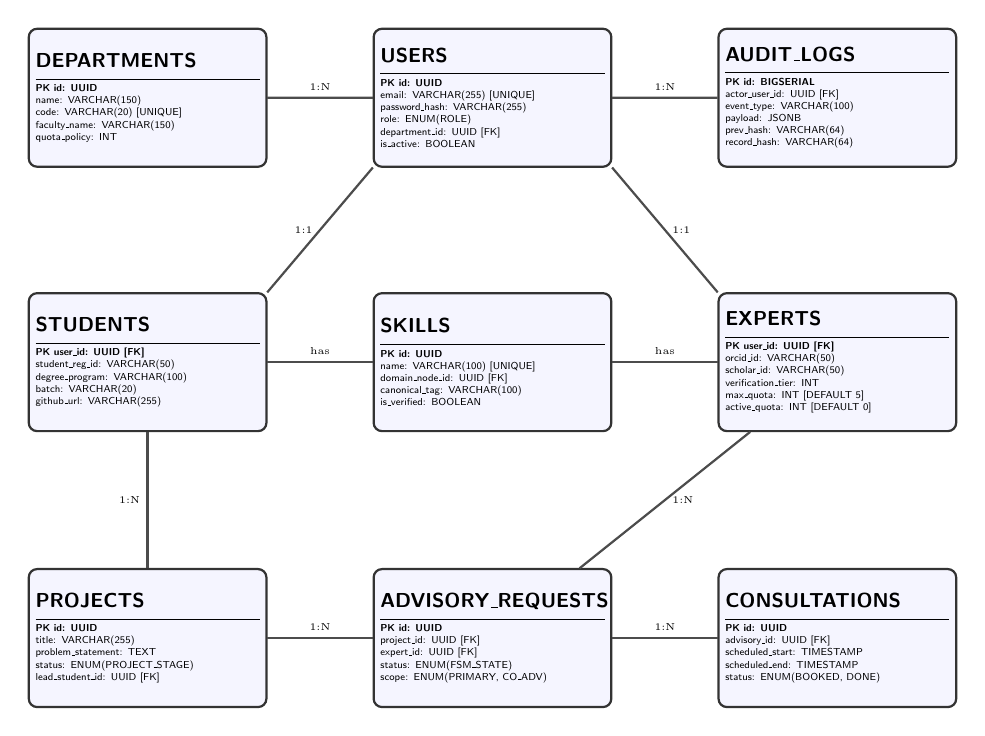
\begin{tikzpicture}[
    scale=0.73, every node/.style={transform shape},
    font=\sffamily\tiny,
    entity/.style={rectangle, draw=black!80, thick, fill=blue!4, text width=3.9cm, minimum height=2.4cm, rounded corners=3pt, align=left},
    rel/.style={thick, draw=black!70}
]

% Row 1: Administrative Governance (y = 6.2)
\node[entity] (dept) at (0, 6.2) {
    \textbf{\normalsize DEPARTMENTS}\\
    \rule{3.9cm}{0.5pt}\\
    \textbf{PK id: UUID}\\
    name: VARCHAR(150)\\
    code: VARCHAR(20) [UNIQUE]\\
    faculty\_name: VARCHAR(150)\\
    quota\_policy: INT
};

\node[entity] (users) at (6.0, 6.2) {
    \textbf{\normalsize USERS}\\
    \rule{3.9cm}{0.5pt}\\
    \textbf{PK id: UUID}\\
    email: VARCHAR(255) [UNIQUE]\\
    password\_hash: VARCHAR(255)\\
    role: ENUM(ROLE)\\
    department\_id: UUID [FK]\\
    is\_active: BOOLEAN
};

\node[entity] (audit) at (12.0, 6.2) {
    \textbf{\normalsize AUDIT\_LOGS}\\
    \rule{3.9cm}{0.5pt}\\
    \textbf{PK id: BIGSERIAL}\\
    actor\_user\_id: UUID [FK]\\
    event\_type: VARCHAR(100)\\
    payload: JSONB\\
    prev\_hash: VARCHAR(64)\\
    record\_hash: VARCHAR(64)
};

% Row 2: User Personas & Taxonomy (y = 1.6)
\node[entity] (students) at (0, 1.6) {
    \textbf{\normalsize STUDENTS}\\
    \rule{3.9cm}{0.5pt}\\
    \textbf{PK user\_id: UUID [FK]}\\
    student\_reg\_id: VARCHAR(50)\\
    degree\_program: VARCHAR(100)\\
    batch: VARCHAR(20)\\
    github\_url: VARCHAR(255)
};

\node[entity] (skills) at (6.0, 1.6) {
    \textbf{\normalsize SKILLS}\\
    \rule{3.9cm}{0.5pt}\\
    \textbf{PK id: UUID}\\
    name: VARCHAR(100) [UNIQUE]\\
    domain\_node\_id: UUID [FK]\\
    canonical\_tag: VARCHAR(100)\\
    is\_verified: BOOLEAN
};

\node[entity] (experts) at (12.0, 1.6) {
    \textbf{\normalsize EXPERTS}\\
    \rule{3.9cm}{0.5pt}\\
    \textbf{PK user\_id: UUID [FK]}\\
    orcid\_id: VARCHAR(50)\\
    scholar\_id: VARCHAR(50)\\
    verification\_tier: INT\\
    max\_quota: INT [DEFAULT 5]\\
    active\_quota: INT [DEFAULT 0]
};

% Row 3: Capstone Projects, Advisory FSM, Consultations (y = -3.2)
\node[entity] (projects) at (0, -3.2) {
    \textbf{\normalsize PROJECTS}\\
    \rule{3.9cm}{0.5pt}\\
    \textbf{PK id: UUID}\\
    title: VARCHAR(255)\\
    problem\_statement: TEXT\\
    status: ENUM(PROJECT\_STAGE)\\
    lead\_student\_id: UUID [FK]
};

\node[entity] (advisory) at (6.0, -3.2) {
    \textbf{\normalsize ADVISORY\_REQUESTS}\\
    \rule{3.9cm}{0.5pt}\\
    \textbf{PK id: UUID}\\
    project\_id: UUID [FK]\\
    expert\_id: UUID [FK]\\
    status: ENUM(FSM\_STATE)\\
    scope: ENUM(PRIMARY, CO\_ADV)
};

\node[entity] (consult) at (12.0, -3.2) {
    \textbf{\normalsize CONSULTATIONS}\\
    \rule{3.9cm}{0.5pt}\\
    \textbf{PK id: UUID}\\
    advisory\_id: UUID [FK]\\
    scheduled\_start: TIMESTAMP\\
    scheduled\_end: TIMESTAMP\\
    status: ENUM(BOOKED, DONE)
};

% Relationships (All orthogonal or direct adjacent lines)
% Top Row connections
\draw[rel] (dept) -- node[above, font=\tiny] {1:N} (users);
\draw[rel] (users) -- node[above, font=\tiny] {1:N} (audit);

% Users to Persona specializations (1:1)
\draw[rel] (users.south west) -- node[left, font=\tiny] {1:1} (students.north east);
\draw[rel] (users.south east) -- node[right, font=\tiny] {1:1} (experts.north west);

% Middle Row connections: Skills to both Students and Experts
\draw[rel] (students) -- node[above, font=\tiny] {has} (skills);
\draw[rel] (skills) -- node[above, font=\tiny] {has} (experts);

% Persona to Project & Advisory
\draw[rel] (students) -- node[left, font=\tiny] {1:N} (projects);
\draw[rel] (experts) -- node[right, font=\tiny] {1:N} (advisory);

% Bottom Row: Projects -> Advisory -> Consultations
\draw[rel] (projects) -- node[above, font=\tiny] {1:N} (advisory);
\draw[rel] (advisory) -- node[above, font=\tiny] {1:N} (consult);

\end{tikzpicture}
\caption{Entity Relationship Diagram (ERD) for UniExpert Data Schema}
\label{fig:erd}
\end{figure}

\clearpage
\section{Class Diagram}
\label{sec:class_diagram}

The object-oriented software design, interface boundaries, and service abstractions are structured in the UML Class Diagram (Figure~\ref{fig:class_diagram}). The diagram is organized into three distinct architectural tiers: Domain Entities, Application and Inference Services, and Infrastructure and Governance Services.

\begin{figure}[H]
\centering
\begin{tikzpicture}[
    scale=0.71, every node/.style={transform shape},
    font=\sffamily\tiny,
    classbox/.style={rectangle, draw=black!80, thick, fill=gray!4, text width=4.1cm, minimum height=2.7cm, rounded corners=3pt, align=left},
    arr/.style={-{Stealth[scale=0.9]}, thick, draw=black!70},
    inher/.style={-{Triangle[open, scale=1.0]}, thick, draw=black!70}
]

% Row 1: Core Domain Entities (y = 6.4)
\node[classbox] (c_project) at (0, 6.4) {
    \textbf{\normalsize Project}\\
    \rule{4.1cm}{0.5pt}\\
    - id: UUID\\
    - title: String\\
    - problemText: String\\
    - stage: ProjectStage\\
    - requiredSkills: Set$<$Skill$>$\\
    \rule{4.1cm}{0.5pt}\\
    + addSkill(s: Skill): Void\\
    + setStage(s: Stage): Void
};

\node[classbox] (c_user) at (6.0, 6.4) {
    \textbf{\normalsize User}\\
    \rule{4.1cm}{0.5pt}\\
    - id: UUID\\
    - email: String\\
    - passwordHash: String\\
    - role: UserRole\\
    - status: AccountStatus\\
    \rule{4.1cm}{0.5pt}\\
    + verifyCredentials(): Boolean\\
    + updateRole(r: UserRole): Void
};

\node[classbox] (c_expert) at (12.0, 6.4) {
    \textbf{\normalsize ExpertProfile}\\
    \rule{4.1cm}{0.5pt}\\
    - orcidId: String\\
    - scholarId: String\\
    - verificationTier: Int\\
    - maxQuota: Int\\
    - activeQuota: Int\\
    \rule{4.1cm}{0.5pt}\\
    + isAvailable(): Boolean\\
    + decrementQuota(): Void
};

% Row 2: Application Services (y = 1.7)
\node[classbox] (c_nlp) at (0, 1.7) {
    \textbf{\normalsize NLPService}\\
    \rule{4.1cm}{0.5pt}\\
    - zeroShotModel: Transformer\\
    - nerModel: TokenClassifier\\
    \rule{4.1cm}{0.5pt}\\
    + extractDomains(text): List\\
    + extractEntities(text): Set\\
    + normalizeTaxonomy(t): List
};

\node[classbox] (c_match) at (6.0, 1.7) {
    \textbf{\normalsize MatchmakingEngine}\\
    \rule{4.1cm}{0.5pt}\\
    - vectorStore: QdrantStore\\
    - weights: ScoringWeights\\
    \rule{4.1cm}{0.5pt}\\
    + queryNearest(vector): List\\
    + computeHybrid(exp, req): Float\\
    + generateXAI(exp, req): Report
};

\node[classbox] (c_fsm) at (12.0, 1.7) {
    \textbf{\normalsize AdvisoryFSMService}\\
    \rule{4.1cm}{0.5pt}\\
    - stateStore: FSMRepository\\
    - timeoutCron: TimerJob\\
    \rule{4.1cm}{0.5pt}\\
    + transition(id, act): State\\
    + checkTimeouts(): Void\\
    + notifyParties(ev): Void
};

% Row 3: Infrastructure & Governance (y = -3.0)
\node[classbox] (c_gap) at (0, -3.0) {
    \textbf{\normalsize SkillGapEngine}\\
    \rule{4.1cm}{0.5pt}\\
    - optimizer: SetCoverSolver\\
    \rule{4.1cm}{0.5pt}\\
    + computeDeficit(p): Set\\
    + recommendCoAdvisors(gap): List\\
    + simulateReadiness(): Float
};

\node[classbox] (c_sched) at (6.0, -3.0) {
    \textbf{\normalsize SchedulerService}\\
    \rule{4.1cm}{0.5pt}\\
    - calendarDb: CalendarRepo\\
    \rule{4.1cm}{0.5pt}\\
    + getOpenSlots(expId): List\\
    + bookSlot(studId, slotId): Bool\\
    + generateICal(b): String
};

\node[classbox] (c_audit) at (12.0, -3.0) {
    \textbf{\normalsize AuditGovernanceService}\\
    \rule{4.1cm}{0.5pt}\\
    - hashLedger: AuditRepository\\
    \rule{4.1cm}{0.5pt}\\
    + logEvent(actor, ev, data): Void\\
    + verifyIntegrity(): Boolean\\
    + exportAccreditationCSV(): File
};

% Connections (100% Zero Intersections)
\draw[inher] (c_expert) -- (c_user);
\draw[arr] (c_project) -- (c_nlp);
\draw[arr] (c_nlp) -- (c_match);
\draw[arr] (c_expert) -- (c_fsm);
\draw[arr] (c_match) -- (c_fsm);

\draw[arr] (c_gap) -- (c_nlp);
\draw[arr] (c_gap) -- (c_match);
\draw[arr] (c_sched) -- (c_match);
\draw[arr] (c_sched) -- (c_fsm);
\draw[arr] (c_fsm) -- (c_audit);

\end{tikzpicture}
\caption{UML Class Diagram for UniExpert Architecture}
\label{fig:class_diagram}
\end{figure}
